\documentclass[12pt]{extarticle}
%Some packages I commonly use.
\usepackage[portuguese]{babel}
\usepackage{graphicx}
\usepackage{framed}
\usepackage[normalem]{ulem}
\usepackage{amsmath}
\usepackage{amsthm}
\usepackage{amssymb}
\usepackage{amsfonts}
\usepackage{enumerate}
\usepackage[utf8]{inputenc}
\usepackage{float}
\usepackage{gensymb}
\usepackage[top=1 in,bottom=1in, left=1 in, right=1 in]{geometry}
\usepackage{multirow}
\usepackage{caption}
\usepackage{subcaption}
\usepackage[utf8]{inputenc}

%A bunch of definitions that make my life easier
\newcommand{\matlab}{{\sc Matlab} }
\newcommand{\cvec}[1]{{\mathbf #1}}
\newcommand{\rvec}[1]{\vec{\mathbf #1}}
\newcommand{\ihat}{\hat{\textbf{\i}}}
\newcommand{\jhat}{\hat{\textbf{\j}}}
\newcommand{\khat}{\hat{\textbf{k}}}
\newcommand{\minor}{{\rm minor}}
\newcommand{\trace}{{\rm trace}}
\newcommand{\spn}{{\rm Span}}
\newcommand{\rem}{{\rm rem}}
\newcommand{\ran}{{\rm range}}
\newcommand{\range}{{\rm range}}
\newcommand{\mdiv}{{\rm div}}
\newcommand{\proj}{{\rm proj}}
\newcommand{\R}{\mathbb{R}}
\newcommand{\N}{\mathbb{N}}
\newcommand{\Q}{\mathbb{Q}}
\newcommand{\Z}{\mathbb{Z}}
\newcommand{\<}{\langle}
\renewcommand{\>}{\rangle}
\renewcommand{\emptyset}{\varnothing}
\newcommand{\attn}[1]{\textbf{#1}}
\theoremstyle{definition}
\newtheorem{theorem}{Theorem}
\newtheorem{corollary}{Corollary}
\newtheorem*{definition}{Definition}
\newtheorem*{example}{Example}
\newtheorem*{note}{Note}
\newtheorem{exercise}{Exercise}
\newcommand{\bproof}{\bigskip {\bf Proof. }}
\newcommand{\eproof}{\hfill\qedsymbol}
\newcommand{\Disp}{\displaystyle}
\newcommand{\qe}{\hfill\(\bigtriangledown\)}
\setlength{\columnseprule}{1 pt}
\usepackage[utf8]{inputenc}

\title{Aula 15 - Leis de Kirchoff}
\author{Felipe Salvador}
\date{Atualizado em \today}

\begin{document}

\maketitle

\section{Introdução}
Uma das formas mais completas de analisar um circuito com diversos elementos elétricos é usando as chamadas \textbf{Leis de Kirchoff}. Ao todo, são 2 leis que conseguem descrever toda a dinâmica de um circuito. Elas foram descobertas e descritas pelo físico alemão Gustav Kirchoff.

\section{1$^a$ Lei de Kirchoff - Lei dos Nós}

A primeira Lei é descrita da seguinte forma: \textbf{Em um nó, a soma de todas as correntes que cheguem ao nó tem que ser igual a soma de todas as correntes que saem do nó, em que um nó é um ponto de saem ramificações de um fio.} A figura a seguir ilustra a ideia:
\begin{figure}[H]
    \centering
    \includegraphics[width=0.6\textwidth]{lei_dos_nós.png}
    \caption{Ilustração da Lei dos Nós - a soma das corrente que chegam no nó tem que ser igual a soma das correntes que saem do nó.}
    \label{fig:lei_dos_no}
\end{figure}

Essa Lei é uma consequência de um dos fundamentos mais básicos da Elétrica: \textbf{não podemos gerar corrente a partir do nada.} Ou seja, caso não haja algum gerador no nó, a corrente tem que ser conservada, logo o que entra é o que sai.

\section{2$^a$ Lei de Kirchoff - Lei das malhas}
A segunda Lei é descrita da seguinte forma: \textbf{Percorrendo uma malha, a soma das diferenças de potenciais (d.d.p.) aplicadas aos equipamentos elétricos tem que ser 0, em que uma malha é um circuito fechado.} Abaixo está a ilustração do conceito:
\begin{figure}[H]
    \centering
    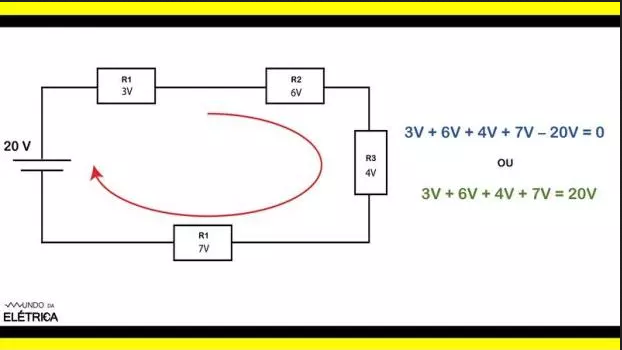
\includegraphics[width=0.8\textwidth]{malha.png}
    \caption{Ilustração da Lei das Malhas - escolha-se um sentido para a malha e soma-se a d.d.p dos componentes do circuito. Essa soma deve ser igual à 0.}
    \label{fig:malha}
\end{figure}
\end{document}
